\documentclass{article}
\usepackage{tikz}
\usetikzlibrary{shapes.geometric, arrows}

\tikzstyle{startstop} = [rectangle, rounded corners, minimum width=3cm, minimum height=1cm,text centered, draw=black]
\tikzstyle{process} = [rectangle, minimum width=3cm, minimum height=1cm, text centered, draw=black]
\tikzstyle{arrow} = [thick,->,>=stealth]

\begin{document}

\begin{center}
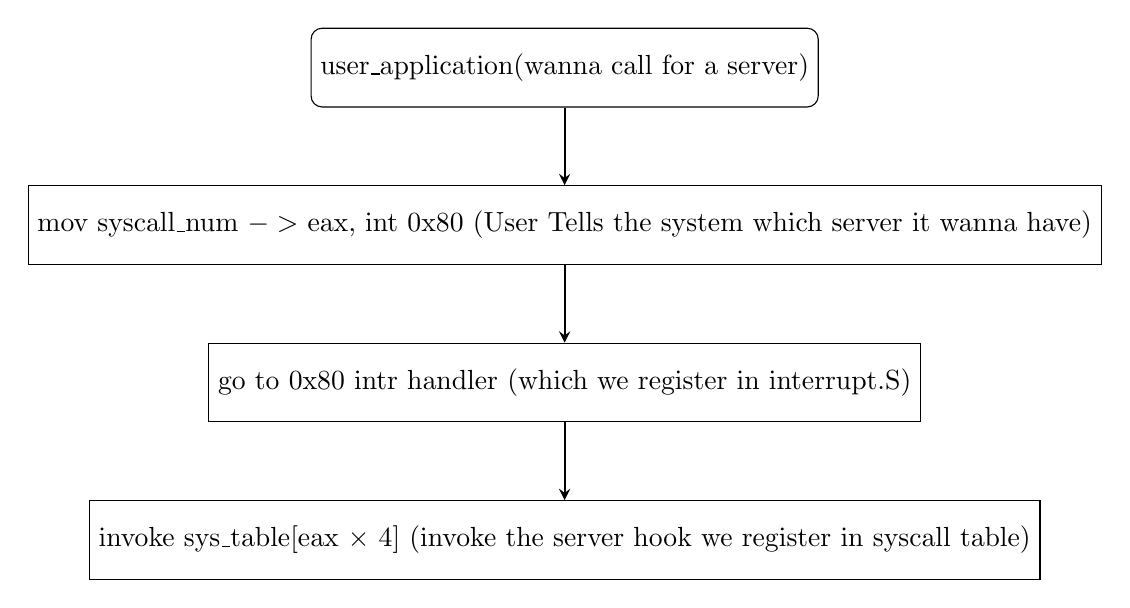
\begin{tikzpicture}[node distance=2cm]

    \node (start) [startstop] {user\_application(wanna call for a server)};
    \node (A) [process, below of=start] {mov syscall\_num $->$ eax, int 0x80 (User Tells the system which server it wanna have)};
    \node (B) [process, below of=A] {go to 0x80 intr handler (which we register in interrupt.S)};
    \node (C) [process, below of=B] {invoke sys\_table[eax $\times$ 4] (invoke the server hook we register in syscall table)};

    \draw [arrow] (start) -- (A);
    \draw [arrow] (A) -- (B);
    \draw [arrow] (B) -- (C);


\end{tikzpicture}
\end{center}

\end{document}
